\chapter{Opis modelu Social Force}
\label{cha:OpisSocialForce}

Model Social Force \cite{SforceModelForPedDyn}, bezsprzecznie najważniejszy z obecnie dostępnych, jest mikrospokowym modelem ciągłym. Zakłada on, że piesi w ruchu mogą zostać w prosty sposób opisani za pomocą sił. Siły te pochodzą nie tylko z oddziaływań konkretnego pieszego na otoczenie, ale także z otoczenia na danego pieszego. Wartość, zwrot oraz kierunek siły finalnej jest składową wszystkich sił działających na danego pieszego. Piesi w modelu reprezentowani są za pomocą cząstek, które dążą do celu w konkretnych kierunkach oraz są pod działaniem wspomnianych sił. Dotychczasowe symulacje komputerowe pokazują, że Model Social Force, pomimo swojej prostoty bardzo realistycznie oddaje rzeczywiste zachowanie tłumu.

\begin{figure}
\centering
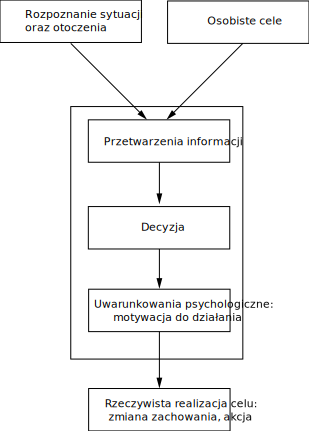
\includegraphics[width=0.5\textwidth]{process.eps}
\caption{Schemat podejmowania decyzji przez pieszego, opracowanie własne na bazie \cite{GuideCrowdDynViaModifiedSocialForceModel}}
\end{figure}

Nie bez znaczenia jest także łatwość uzyskania parametrów oraz wartości potrzebnych do symulacji. Wartości takie jak predkość $\vec{v_{\alpha}}$ czy położenie $\vec{r_{\alpha}}$ danego pieszego $\alpha$ są łatwe do obliczenia, ale także do skalibrowania z danami empirycznymi.

Pierwsze symulacje korzystające z modelu SF były skupione głównie na ewakuacjach budynków. W tego typu sytuacjach celem pieszego jest dojście do wyjścia w możliwie najkrótszym czasie. Obecnie istnieje mnogość wariantów modelu, które pozwalają na zamodelowanie większej ilości zachowań. Obecne modyfikacje przewidują przykładowo unikanie "spychania" innych uczestników ruchu poprzez pieszych poruszających się z większą prędkością \cite{6}.

Istnieje bardzo wiele różnych modyfikacji modelu Social Forca. Wykorzystany w pracy model \cite{GuideCrowdDynViaModifiedSocialForceModel} bazuje na oryginalnym modelu Helbinga \cite{SforceModelForPedDyn} zakłada, że na pieszego działają trzy siły. Desired force $\vec{f_{i}^{0}}$, siła interakcji pomiędzy pieszymi $i$ oraz $j$, $\vec{f_{ij}}$ oraz siła interakcji pomiędzy pieszym $i$, a przeszkodami, $\vec{f_{iw}}$

Siła działająca na każdego z pieszych definiuje się jako:

\begin{equation}
m_{i} \frac{d\vec{v_{i}}(t)}{dt} = \vec{f_{i}^{0}} + \sum_{j(\neq i)} \vec{f_{ij}} + \sum _{w} \vec{f_{iw}}
\end{equation}

gdzie
\begin{eqwhere}[2cm]
	\item[$m_{i}$] masa pieszego $i$
	\item[$\vec{v}_{i}(t)$] aktualna prędkość
\end{eqwhere}

\section{Desired force}
\label{sec:desiredForce}

Bazując na obserwacjach można wywnioskować, że piesi wykazują niechęć do zmiany prędkości oraz kierunku swojej drogi. Zazwyczaj wybierana jest droga, którą można podążać prosto przez jak najdłuższy okres czasu, nawet jeśli drogi alternatywne są takiej samej długości, a droga wybrana przez pieszego jest mocno zatłoczona. Kierunek ruchu obliczany jest na podstawie wzoru:

\begin{equation}
\vec{e}_{\alpha}(t) = \frac{\vec{r}_{\alpha}^{k} - \vec{r}_{\alpha}(t)}{\parallel \vec{r}_{\alpha}^{k} - \vec{r}_{\alpha}(t) \parallel}
\end{equation}

gdzie
\begin{eqwhere}[2cm]
	\item[$e_{\alpha}(t)$] aktualna pozycja pieszego $\alpha$ w czasie $t$
	\item[$\vec{r}_{\alpha}^{k}$] najbliższy punkt na ścieżce do celu
\end{eqwhere}

\begin{figure}
\centering
\includegraphics[width=0.5\textwidth]{desiredforce2.eps}
\caption{Schemat siły \textit{desired force} , opracowanie własne na bazie \cite{AMSFMfPBSaSC}}
\end{figure}

\begin{figure}
\centering
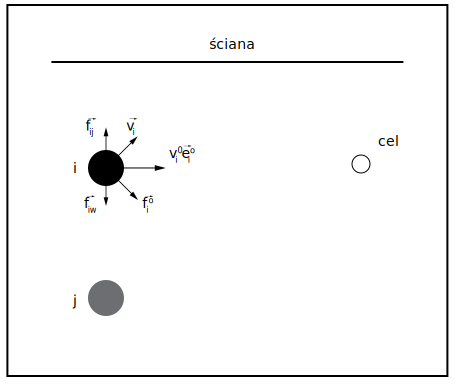
\includegraphics[width=0.5\textwidth]{desiredforce.eps}
\caption{Diagram modelu Social Force, opracowanie własne na bazie \cite{GuideCrowdDynViaModifiedSocialForceModel}}
\end{figure}

W przypadku kiedy ruch pieszego odbywa się bez przeszkód porusza się on w kierunku pozycji celu, z preferowaną przez siebie prędkością, $\vec{v_{i}^{0}}$. Z powodu działania na pieszego sił~z otoczenia, obserwuje się dążenie pieszego do osiągnięcia preferowanej przez siebie prędkości w czasie relaksacji $\tau$.

\begin{equation}
\vec{f}_{i}^{0} = m_{i} \frac{v_{i}^{0}(t) \vec{e_{i}^{0}} - \vec{v_{i}}(t)}{\tau}
\end{equation}

gdzie
\begin{eqwhere}[2cm]
	\item[$\vec{v_{i}^{0}}$] wartość domyślnej prędkości pieszego
	\item[$\vec{e_{i}^{0}}$] kierunek ruchu jaki pieszy chce osiągnąć
	\item[$\tau$] czas relaksacji
\end{eqwhere}
	
Jest to tzw. \textit{desired speed} [wyjaśnić], odzwierciedla ona dążenie danego pieszego $i$ do osiągnięcia preferowanej prędkości.

Domyślna prędkość pieszego przyjmuje zazwyczaj wartość około $1.34 \frac{m}{s^{2}}$ z odchyleniem standardowym $0.26 \frac{m}{s^{2}}$ \cite{HeBuAjTw}

\section{Interakcja pomiędzy pieszymi}
\label{sec:interactionBetweenPedestrians}

Naturalnym jest, że kiedy zbliżamy się do innych uczestników ruchu czujemy się niekomfortowo. Zakłada się, że każdy z pieszych, który jest w konflikcie z innym uczestnikiem ruchu generuje wokół siebie eliptyczne pole siły, które działa na drugiego z pieszych. Aby uniknąć wypadków utrzymują dystans pomiędzy innymi uczestnikami ruchu oraz przeszkodami. Dystans ten zmniejsza się w przypadku kiedy pieszy śpieszy się oraz kiedy wzrasta gęstość tłumu. Gęstość tłumu zwiększa się w szczególności kiedy piesi znajdują się w okolicy miejsc wywierających zainteresowanie oraz w wąskich przejściach. Siła interakcji pomiędzy pieszymi $i$ oraz $j$, $\vec{f_{ij}}$ definiowana jest jako suma dwóch sił, socjologiczno-psychologicznej oraz fizycznej. Piesi mogą także formować grupy, których zachowanie można później sprowadzić do opisu pojedynczego agenta \cite{HeBuAjTw}

\begin{equation}
\vec{f_{ij}} = \vec{f}_{ij}^{s} + \vec{f}_{ij}^{p}
\end{equation}
Pierwsza z nich $\vec{f_{ij}^{s}}$ związana jest z naturalnym ludzkim odruchem utrzymywania dystansu od drugiego człowieka. Przyjmuje ona wartość maksymalną, gdy odległość między dwoma pieszymi $d_{ij}$ maleje, a wartość mniejszą w przypadku oddalania się pieszych.

\begin{equation}
\vec{f_{ij}^{s}} = A_{i} exp[(r_{ij} - d_{ij}) / B_{i}]\vec{n_{ij}}
\end{equation}

gdzie
\begin{eqwhere}[2cm]
	\item[$A_{i}$] Moc siły
	\item[$B_{i}$] Dystans działania siły
	\item[$\vec{n_{ij}}$] wektor jednostkowy o początku w centrum strefy prywatnej pieszego $i$ a końcu w centrum tej strefy pieszego $j$
\end{eqwhere}

Druga z sił $\vec{f_{ij}^{p}}$ wywiera nacisk na pieszych kiedy dystans pomiędzy dwoma pieszymi, $d_{ij}$ jest mniejszy od sumy promieni ich stref prywatnych $r_{ij} = r_{i} + r_{j}$. Siła ta składa się z "body force", $\vec{f} _{ij}^{p_{1}}$ oraz \textit{sliding friction force}, $\vec{f} _{ij}^{p_{2}}$.

\begin{equation}
\vec{f}_{ij}^{p} = kg(r_{ij} - d_{ij}) \vec{n}_{ij} + \kappag (r_{ij} - d_{ij}) \Delta v _{ij}^{t} \vec{t}_{ij}
\end{equation}

gdzie
\begin{eqwhere}[2cm]
	\item[$k$] body compression coefficient
	\item[$\kappa$] Coeficient of sliding friction
	\item[$\vec{n}_{ij}$] wektor jednostkowy o początku w pozycji pieszego $i$ a końcu w pozycji pieszego $j$
	\item[$\Delta v_{ij}^{t} * \vec{t}_{ij}$] zmiana prędkości wzdłuż stycznej do eliptycznego pola strefy prywatnej
\end{eqwhere}

\begin{equation}
g(x) = \lbrace {0, if x < 0, x if x \geq 0.}
\end{equation}

Warto zaznaczyć, że druga z sił przyjmuje pewne wartości nawet w przypadku kiedy dwoje pieszych znajduje się daleko od siebie. Oznacza to, że piesi zawsze starają się utrzymać dystans od siebie nawzajem \cite{relativeVelocity}.


\section{Zalety oraz wady Modelu Social Foce}

Największą z zalet opisywanego modelu jest precyzja odwzorowania zachowań mikroskopowych oddziaływań pomiędzy pieszymi oraz otaczającą ich rzeczywistością. SFM pokazuje także wiele znanych zachowań takich jak:

\begin{itemize}
\item Unikanie kontaktu z przeszkodami oraz innymi uczestnikami ruchu przed dojściem do kolizji,
\item \textit{Szybciej znaczy wolniej}, im szybciej pieszy próbuje się poruszać tym bardziej zatłoczone stają się miejsca takie jak obszary wyjścia z budynków co skutkuje spowolnieniem ruchu,
\item formowanie strug, w korytarzach piesi próbują poruszać się w liniach. Zachowanie to może być zauważone w szczególności kiedy dwie grupy ludzi poruszają się w przeciwnych kierunkach.
\end{itemize}
Wśród wielu zalet modelu możemy wskazać także wady. Pierwszą z nich jest mała wydajność obliczeniowa oraz trudności z odwzorowaniem niektórych sytuacji. Mnogość sił, które są obliczane w przemnożeniu poprzez ilość pieszych powoduje wysoki narzut na ilość obliczeń. W tym miejscu dużą konkurencją stają się automaty komórkowe, które nie wymagają tak skomplikowanych obliczeń dając jednocześnie szerokie spektrum odwzorowania zróżnicowanych zachowań ruchu pieszych.
